\chapter*{Projekt aplikacji}
Aplikacja jest wysoce wyspecjalizowana -- przeprowadza wyłącznie proces symulacji i uczenia. Użytkownik może konfigurować ustawienia tego procesu.
\section*{Wymagania funkcjonalne}
\begin{itemize}
	\item Przeprowadzenie procesu uczenia optymalnych czasów świecenia sygnalizatorów na skrzyżowaniu za pośrednictwem algorytmu ewolucyjnego,
	\item Konfiguracja ustawień symulacji, będącej bazą procesu uczenia,
	\item Konfiguracja ustawień algorytmu ewolucyjnego,
	\item Wyświetlanie na bieżąco informacji o przebiegu uczenia,
	\item Wyświetlenie wyników uczenia po jego zakończeniu.
\end{itemize}
\section*{Wymagania pozafunkcjonalne}
\begin{itemize}
	\item Stabilność -- aplikacja musi pracować bezawaryjnie przez wiele godzin,
	\item Wydajność -- aplikacja musi działać na tyle wydajnie, aby symulacja mogła być przeprowadzana kilkadziesiąt razy szybciej niż czas rzeczywisty.
\end{itemize}
\begin{figure}
	\centering
	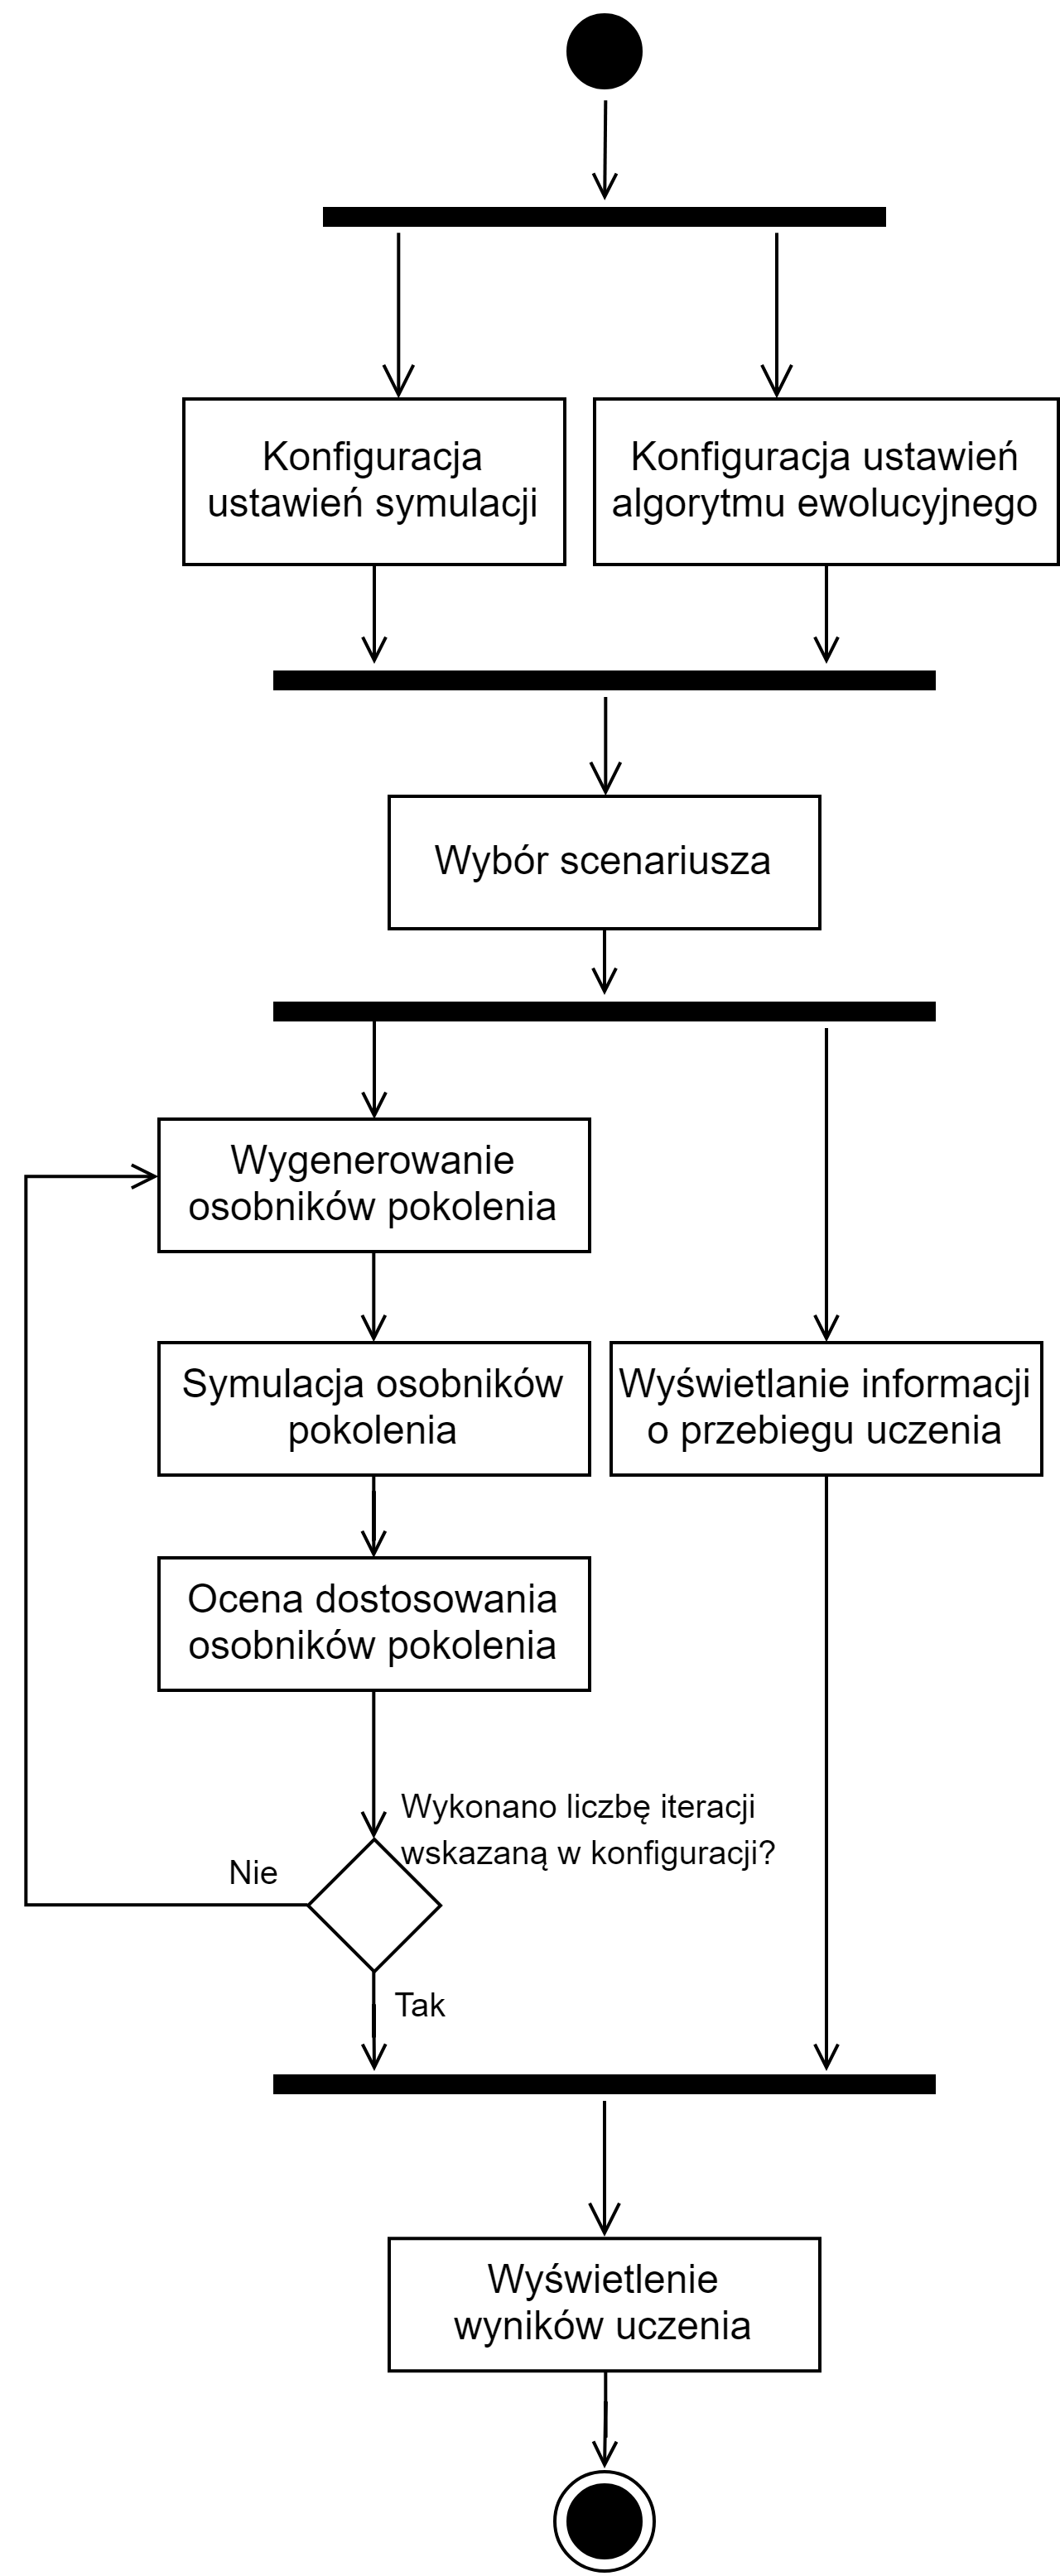
\includegraphics[height=0.9\textheight]{diagram_aktywnosci}
	\caption[Diagram aktywności przypadku użycia ,,Przeprowadź proces uczenia sygnalizacji'']{Diagram aktywności przypadku użycia ,,Przeprowadź proces uczenia sygnalizacji''}
	\label{fig:diagramaktywnosci}
\end{figure}
\section*{Przypadki użycia}
W projekt występuje tylko jeden przypadek użycia: ,,Przeprowadź proces optymalizacji sygnalizacji świetlnej''. Przedstawia go diagram aktywności na rysunku~\ref{fig:diagramaktywnosci}. 
\section*{Przebieg przypadku użycia ,,Przeprowadź proces optymalizacji sygnalizacji świetlnej''}
Użytkownik najpierw może ustawić konfigurację symulacji oraz algorytmu ewolucyjnego. Następne wybiera scenariusz (czyli kolejność zapalania się sygnalizatorów) co powoduje rozpoczęcie procesu uczenia. Aplikacja kolejno generuje, symuluje, a potem ocenia osobników pokolenia, jednocześnie wyświetlając na ekranie informacje o przebiegu uczenia. Pokolenia są kolejno generowane tak długo, aż zostanie osiągnięta ich liczba określona w konfiguracji. Następnie aplikacja wyświetla ekran końcowy prezentujący wyniki uczenia.
%\begin{table}
%	\caption{Scenariusz przypadku użycia ,,Przeprowadź proces optymalizacji sygnalizacji świetlnej''}
%	\begin{tabularx}{\textwidth}{|l|X|}
%		\hline 
%		Nazwa & Przeprowadź proces optymalizacji sygnalizacji świetlnej \\ 
%		\hline 
%		Aktorzy & Użytkownik \\ 
%		\hline 
%		Opis & Funkcja pozwala użytkownikowi wywołać proces optymalizacji sygnalizacji świetlnej na skrzyżowaniu \\ 
%		\hline
%		Warunki początkowe & brak \\
%		\hline 
%		Główny przepływ zdarzeń & 
%		1. Użytkownik wprowadza ustawienia symulacji w menu głównym\newline
%		2. Użytkownik wprowadza ustawienia algorytmu ewolucyjnego w menu głównym\\ 
%		\hline
%		Warunki końcowe & Zakończono proces optymalizacji i wyświetlono wyniki uczenia \\
%		\hline
%	\end{tabularx} 
%	\label{tab:scenariusz}
%\end{table}
